\documentclass[a4paper]{article}
\usepackage[utf8]{inputenc}
\usepackage[L7x]{fontenc}
\usepackage[lithuanian]{babel}
\usepackage{lmodern}
\usepackage{graphicx}
\usepackage[top=2cm, bottom=2cm, left=1.5cm, right=1.5cm, footskip=1cm, a4paper]{geometry}
\usepackage{indentfirst}
\usepackage{framed}
\usepackage{tikz}
\usepackage{listofitems}
\usepackage{xcolor}
\usepackage{verbatim}
\usepackage[unicode]{hyperref}
\usepackage{amsmath,amsfonts,amssymb,amsthm}
\usepackage{minted}
%\usepackage{mathptmx}
\usepackage{calc}
\usetikzlibrary{tikzmark,calc,,arrows,shapes,decorations.pathreplacing}
\tikzset{every picture/.style={remember picture}}
\usepackage{accents}
\newcommand\myubar[1]{%
\underaccent{\bar}{#1}}
\graphicspath{{"/Users/Vartotojas/Desktop/EnolaProject/Kodinimas/Pythoning/demo - create folder of images problems in pdf/"}}
\renewenvironment{framed}[1][\hsize]
   {\MakeFramed{\hsize#1\advance\hsize-\width \FrameRestore}}%
   {\endMakeFramed}

\newcommand{\inc}[1]{\includegraphics[width=\textwidth]{#1}}

%use python script:
%lines='''B2002_5, B2002_4'''
%print(', '.join([n[1:5]+'/'+n[0:5]+'/'+n+'.jpg' for n in lines.replace(" ", "").split(',')]))

\begin{document}
\tableofcontents
\newpage
\textit{- Prieš akis matome veiksmą $3\times 5$. Kokia galėtų būti kairėje parašyto skaičiaus prasmė?}

\textit{- Trys.}

\textit{- Tai reikšmė, o ne prasmė. Tačiau prasmę galima suvokti, jei žinai, kur gyvenime $3\times 5$ pasitaikė}

\section{Šiame straipsnyje įvestų sąvokų žodynėlis}

\colorbox{green}{Matematinis supratimas} - tai sugebėjimas \fbox{matematinę medžiagą} įsiminti taip, kad ji būtų kuo geriau atkuriama atmintyje ilguoju mokymosi laikotarpiu.

\colorbox{green}{Matematinis vaizdinys} - tai prasmės, kurias moksleivis geba suteikti duoto simbolinio užrašo elementams. Pavyzdžiai:

\phantom{xxxxxxxxxxxxxxxxxxxx}$\tikz[baseline]{\node(d1) {(-3)}} \times \tikz[baseline]{\node(d2){(-5)}} = \tikz[baseline]{\node(d3) {15}}$
\begin{tikzpicture}[remember picture, overlay] %overlay parametras nurodo, kad paveikslėlis eis tiesiai iš lygties
%in yra įėjimo kampas, out yra išėjimo kampas (kur eis vektorius, priešingas įėjimo krypčiai; išėjimo krypties kampas)
%dėmenyje skliausteliuose: (pirmas narys= kampas, kuriuo slinksis tekstas; antras narys = jo nuotolis)
%atskaitos tašką nurodo north - t.y. kad rodyklė eis iš po teksto
%text width= paaiškinamo teksto plotis, align=center garantuoja, kad kėlimas į kitą eilutę leistinas
\draw[blue,thick,->] (d1) to [in=90,out=265] + (225:1.7cm) node[anchor=north,text = black, align=center] {kiek kartų atsisakiau \\ pirkti \textit{Rafaello}};
\draw[blue,thick,->] (d2) to [in=90,out=265] + (270:0.7cm) node[anchor=north,text = black, align=center] {kokia \textit{Rafaello} kaina};
\draw[blue,thick,->] (d3) to [in=90,out=265] + (315:1.7cm) node[anchor=north,text = black, align=center] {kaip pakito \\ mano lėšos};
\end{tikzpicture}
\phantom{xxxxxxxxxxxxxxxxxxxxxxxxx}$\tikz[baseline]{\node(d4) {-5}} + \tikz[baseline]{\node(d5){(-3)}} = \tikz[baseline]{\node(d6) {-8}}$
\begin{tikzpicture}[remember picture, overlay] %overlay parametras nurodo, kad paveikslėlis eis tiesiai iš lygties
%in yra įėjimo kampas, out yra išėjimo kampas (kur eis vektorius, priešingas įėjimo krypčiai; išėjimo krypties kampas)
%dėmenyje skliausteliuose: (pirmas narys= kampas, kuriuo slinksis tekstas; antras narys = jo nuotolis)
%atskaitos tašką nurodo north - t.y. kad rodyklė eis iš po teksto
%text width= paaiškinamo teksto plotis, align=center garantuoja, kad kėlimas į kitą eilutę leistinas
\draw[blue,thick,->] (d4) to [in=90,out=265] + (225:1.9cm) node[anchor=north,text = black, align=center] {kaip pakito \\ temperatūra naktį};
\draw[blue,thick,->] (d5) to [in=90,out=265] + (270:0.7cm) node[anchor=north,text = black, align=center] {kaip pakito \\ temperatūra dieną};
\draw[blue,thick,->] (d6) to [in=90,out=265] + (315:1.9cm) node[anchor=north,text = black, align=center] {kaip pakito \\ temperatūra iš viso};
\end{tikzpicture}
 \\ \\ \\ \\ \\ \\ \\
\phantom{xxxxxxxxxxxxxxxxxxxx}$\frac{\tikz[baseline]{\node(d7) {50}}}{\tikz[baseline]{\node(d8){14}}} = \tikz[baseline]{\node(d9) {$3\frac{8}{14}$}}$
\begin{tikzpicture}[remember picture, overlay] %overlay parametras nurodo, kad paveikslėlis eis tiesiai iš lygties
%in yra įėjimo kampas, out yra išėjimo kampas (kur eis vektorius, priešingas įėjimo krypčiai; išėjimo krypties kampas)
%dėmenyje skliausteliuose: (pirmas narys= kampas, kuriuo slinksis tekstas; antras narys = jo nuotolis)
%atskaitos tašką nurodo north - t.y. kad rodyklė eis iš po teksto
%text width= paaiškinamo teksto plotis, align=center garantuoja, kad kėlimas į kitą eilutę leistinas
\draw[blue,thick,->] (d7) to [in=90,out=180] + (225:2.5cm) node[anchor=north,text = black, align=center] {ką dalijame};
\draw[blue,thick,->] (d8) to [in=90,out=225] + (270:0.7cm) node[anchor=north,text = black, align=center] {į kiek dalių};
\draw[blue,thick,->] (d9) to [in=90,out=265] + (315:1.7cm) node[anchor=north,text = black, align=center] {kas gavosi};
\end{tikzpicture}
\phantom{xxxxxxxxxxxxxxxxxxxxxxxxx}$\tikz[baseline]{\node(d10) {7}} \tikz[baseline]{\node(d11){$x$}} + \tikz[baseline]{\node(d12){20}} = \tikz[baseline]{\node(d13) {34}}$
\begin{tikzpicture}[remember picture, overlay] %overlay parametras nurodo, kad paveikslėlis eis tiesiai iš lygties
%in yra įėjimo kampas, out yra išėjimo kampas (kur eis vektorius, priešingas įėjimo krypčiai; išėjimo krypties kampas)
%dėmenyje skliausteliuose: (pirmas narys= kampas, kuriuo slinksis tekstas; antras narys = jo nuotolis)
%atskaitos tašką nurodo north - t.y. kad rodyklė eis iš po teksto
%text width= paaiškinamo teksto plotis, align=center garantuoja, kad kėlimas į kitą eilutę leistinas
\draw[blue,thick,->] (d10) to [in=90,out=265] + (225:2.5cm) node[anchor=north,text = black, align=center] {Kiek stalų lauke};
\draw[blue,thick,->] (d11) to [in=90,out=265] + (270:0.7cm) node[anchor=north,text = black, align=center] {Po kiek žmonių \\ prie kiekvieno \\ stalo lauke};
\draw[blue,thick,->] (d12) to [in=90,out=265] + (315:1.9cm) node[anchor=north,text = black, align=center] {Kiek žmonių \\ kavinės viduje};
\draw[blue,thick,->] (d13) to [in=160,out=350] + (350:1.9cm) node[anchor=west,text = black, align=center] {Kiek žmonių \\ visoje kavinėje};
\end{tikzpicture}
 \\ \\ \\ \\ \\ \\ \\

\colorbox{green}{Matematinio vaizdinio suvokimas} - tai prasmių priskyrimas simboliniame matematikos užraše esantiems nariams. Suvokimas gali būti teisingas arba klaidingas. Laikysime, jog teisingai suvokti vaizdiniai spartina tolimesnį mokymosi procesą ir didina tolimesnę mokymosi motyvaciją, o klaidingai suvokti vaizdiniai stabdo mokymosi procesą ir mažina tolimesnę mokymosi motyvaciją. Pavyzdžiui moksleivis gali suvokti, jog užraše $\frac{50}{14}$ skaičius $14$ nurodo picos gabaliukų kiekį, o $50$ nurodo, į kiek dalių dalijama pica, tačiau šis vaizdinys yra suvoktas klaidingai. Taip pat vaizdinys gali būti ir nesuvoktas - simbolinio užrašo nariams nepriskiriamos jokios prasmės.

\colorbox{green}{Matematinio vaizdinio atkūrimas} - tai procesas, kuomet remiantis tam tikru suvokimu atmintyje yra atkuriamos vaizdinio prasmės.

\colorbox{green}{Pradinis matematinio vaizdinio atkūrimo sudėtingumas} - tai vaizdinio, suvokto po pirmos pažinties su vaizduojamu objektu, atkūrimo atmintyje sudėtingumas vertinant jį intuityviai arba pagal moksliniais tyrimais grįstą požiūrį.

\colorbox{green}{Matematinį vaizdinį} laikysime \colorbox{green}{papildančiu kitą}, jeigu norint patvirtinti jo suvokimo teisingumą galima remtis prasmėmis, suvoktomis ankstesniame vaizdinyje. Pavyzdžiui bendravardiklininant dvi trupmenas reikia suvienodinti jų vardiklius ir gautas trupmenas sudėti. Tokios procedūros atkūrimas atmintyje ilguoju laikotarpiu reikalauja šių dviejų vaizdinių suvokimo: 1) taisyklės $\frac{a}{b}=\frac{ak}{bk}$ vaizdinio; 2) mažiausio bendrojo kartotinio sąvokos vaizdinio (kokia užrašo $MBK(a,b)$ prasmė ir simbolių $a$, $b$ prasmė?) 

\colorbox{green}{Matematinį vaizdinį} laikysime \colorbox{green}{išvestu iš kito}, jeigu norint patvirtinti jo suvokimo teisingumą ne tik galima remtis prasmėmis, suvoktomis ankstesniame vaizdinyje, bet ir neišvengiama (suvokiančiajam vaizdinį).

-------------------------------------------------------------------------------------------------------------------------------------

\colorbox{green}{Matematinio vaizdinio suvokimą} laikysime \colorbox{green}{konkrečiu}, jeigu jis suvokiamas remiantis gyvenimiškose situacijose iškylančiomis tikroviškų objektų prasmėmis. Pavyzdžiui mažiausio bendrojo kartotinio sąvokos vaizdinys konkretus, nes užraše $MBK(a,b)$ skaičiui $a$ galime priskirti prasmę  ,,per kiek minučių apibėga ratą pirmas bėgikas", skaičiui $b$ - ,,per kiek minučių apibėga ratą antras bėgikas", o rezultatui $MBK(a,b)$ - ,,po kiek laiko jie susitiks starto vietoje, jei startavo vienodu metu". 

\colorbox{green}{Matematinio vaizdinio suvokimą} laikysime \colorbox{green}{abstrakčiu}, jeigu jis suvokiamas remiantis abstrakcijomis, tokiomis, kaip kiekis, skaičius, šaknis, dėmuo ir pan. Pavyzdyje matyti, jog lygybės $7^2\times 7^3=7^5$ vaizdinio suvokimas yra abstraktus:

\phantom{xxxxxxxxxxxxxxxxxxxxxxxxx}$\tikz[baseline]{\node(d14) {$7$}}\tikz[baseline]{\node(d15){$^2$}} \times \tikz[baseline]{\node(d16){7}}\tikz[baseline]{\node(d17) {$^3$}}=\tikz[baseline]{\node(d18) {$7$}}\tikz[baseline]{\node(d19){$^5$}}$
\begin{tikzpicture}[remember picture, overlay] 

%overlay parametras nurodo, kad paveikslėlis eis tiesiai iš lygties
%in yra įėjimo kampas, out yra išėjimo kampas (kur eis vektorius, priešingas įėjimo krypčiai; išėjimo krypties kampas)
%dėmenyje skliausteliuose: (pirmas narys= kampas, kuriuo slinksis tekstas; antras narys = jo nuotolis)
%atskaitos tašką nurodo north - t.y. kad rodyklė eis iš po teksto
%text width= paaiškinamo teksto plotis, align=center garantuoja, kad kėlimas į kitą eilutę leistinas
\draw[blue,thick,->] (d14) to [in=90,out=265] + (225:2.5cm) node[anchor=north,text = black, align=center] {daugiklis};
\draw[blue,thick,->] (d16) to [in=60,out=225] + (215:3cm) node[anchor=west,text = black, align=center] {};
\draw[blue,thick,->] (d18) to [in=40,out=205] + (208:3.9cm) node[anchor=west,text = black, align=center] {};
\draw[blue,thick,->] (d15) to [in=90,out=265] + (300:1.9cm) node[anchor=north,text = black, align=center] {kiek kartų daugiklis \\ pasikartoja pirmąsyk};
\draw[blue,thick,->] (d17) to [in=160,out=350] + (340:1.7cm) node[anchor=north,text = black, align=center] {kiek kartų daugiklis \\ pasikartoja antrąsyk};
\draw[blue,thick,->] (d19) to [in=190,out=350] + (350:2.7cm) node[anchor=west,text = black, align=center] {kiek kartų daugiklis \\ pasikartoja iš viso};
\end{tikzpicture}
\\ \\ \\ \\ \\ \\ \\

Iš šio pavyzdžio matyti dar ir kitas dalykas: šis vaizdinys yra išvestas iš laipsnio vaizdinio, nes neturint teisingo laipsnio matematinio vaizdinio suvokimo, nebūtų galima suvokti, kaip reiškinys $7^2$ yra susijęs su daugiklio 7 pasikartojimu dusyk. Beje, reiškinys $7^2$ turi ir abstraktų (7 siejamas su daugikliu), ir konkretų vaizdinį (7 siejamas su kvadrato kraštinės ilgiu).

\colorbox{green}{Matematinio vaizdinio suvokimą} laikysime \colorbox{green}{simboliniu}, jeigu simboliams nesuteikiamos kitokios prasmės, nei jų vieta simboliniame matematinio objekto užraše. Pavyzdžiui lygybės $\frac{1}{2}-\frac{1}{3}=\frac{3}{6}-\frac{2}{6}$ simbolinis suvokimas būtų toks: kairėje lygybės pusėje vienetai yra skaičiai, esantys viršuje, 2 ir 3 yra skaičiai, esantys apačioje, dešinėje pusėje 6 yra kairės pusės apatinių skaičių sandauga, o 3 ir 2 yra tam tikrų kairėje pusėje esančių simbolių sandaugos.

-------------------------------------------------------------------------------------------------------------------------------------

\colorbox{green}{Matematinį vaizdinį} laikysime \colorbox{green}{abstrakčiu}, jeigu jis negali būti suvoktas konkrečiai. 

\colorbox{green}{Matematinį vaizdinį} laikysime \colorbox{green}{konkrečiu}, jeigu jis gali būti suvoktas ir konkrečiai, ir abstrakčiai, tačiau pradinis konkretaus vaizdinio sudėtingumas yra mažesnis už pradinį abstraktaus vaizdinio sudėtingumą.

\colorbox{green}{Matematinį vaizdinį} laikysime \colorbox{green}{simboliniu}, jeigu jo simbolinio suvokimo sudėtingumas yra mažesnis už kitaip suvokto vaizdinio sudėtingumą.

\colorbox{green}{Matematinį vaizdinį} laikysime \colorbox{green}{konfliktišku}, jeigu su vienomis simbolinio užrašo reikšmėmis vaizdinys negali būti suvokiamas taip, kaip su kitomis. Pavyzdžiui su laipsnio $n$ reikšmėmis, lygiomis 1, 2 ir 3, skaičiaus $7^n$ prasmė gali būti suvokta kaip tam tikros srities dydis, o su didesnėmis reikšmėmis negali. Be to su natūraliosiomis $n$ reikšmėmis šio skaičiaus prasmė gali būti suvokta kaip $n$ daugiklių daugyba, o su kitomis negali. Taip pat lygties $7x+20=34$ sprendimo vaizdinys gali būti siejamas su svarstyklėse atliekamais veiksmais (su sąlyga, kad jos pusiausvyros), o lygties $7x-20=36$ negali.

-------------------------------------------------------------------------------------------------------------------------------------

\colorbox{green}{Matematinio vaizdinio abstrakcija} vadinsime tokį suvokimą, kuris yra teisingas ir persidengia su grupe kitų konkrečiai suvokiamų vaizdinių, be to, tinka jiems išvesti. Pavyzdžiui tiek laipsnio $7^4$, tiek sandaugos $4\times 7$ vaizdinius galima abstrahuoti ligi vieno vaizdinio, jei abu ketvertus laikysime ,,elementų pasikartojimo kiekiu", o septynetus ,,pasikartojančiais elementais" (šiuo tikslu matematikoje įvesta grupės sąvoka).

\colorbox{green}{Matematiniu portretu} vadinsime visų matematinių vaizdinių, kurie gali būti įtraukti į teisingą simbolinio užrašo, taisyklės ar uždavinio sprendimo paaiškinimą, visumą.

\colorbox{green}{Matematiniu paveikslu} vadinsime tą patį, tik paaiškinimai kyla besimokančiojo galvoje ir yra nebūtinai teisingi.

\colorbox{green}{Matematinio portreto fokusu} vadinsime uždavinio sprendimo, taisyklės įrodymo ar tam tikro įsiminimo būdo dalyje esantį vaizdinį, kurį uždavinio sprendimo ar taisyklės atkūrimo metu intuityviai pamatyti atrodo sudėtingiausia. Pvz. Skirtingais skaitmenimis užrašomo devynženklio skaičiaus skaitmenų suma lygi 40 reikia nustatyti tokio skaičiaus skaitmenų sandaugą. Kokius dalykus reikia suvokti šiame uždavinyje? Kokie jų vaizdiniai? Kurio vaizdinio sudėtingumas gerokai išsiskiria iš kitų?

Šiame tekste \colorbox{green}{žalia spalva} žymimos naujos sąvokos, \colorbox{orange}{oranžine spalva} žymimos temos, įeinančios į mokyklinį turinį, \colorbox{pink}{rožine spalva} žymimi gebėjimai, kurių reikia norint suprasti mokyklinį turinį.

\section{Tyrimo metodika}

Pagrindinis tyrimo tikslas yra kuo tikslesnis nustatymas, kokias kompetencijas reiktų ugdyti norint, jog matematikos mokomoji medžiaga būtų kuo geriau atkuriama atmintyje ilguoju mokymosi laikotarpiu. Mano paties penkerius metus siekianti matematikos mokymo patirtis rodo, jog klasikinis matematikos mokymasis, kuomet stengiamasi įveikti kuo daugiau uždavinių iš vadovėlio arba uždavinynų, dažniausiai juos darant pagal analogijas su kitais uždaviniais, tokia prasme yra neproduktyvus. Trumpai tariant, toks mokymasis apsiriboja metodais, kuomet stengiamasi kuo geriau prisiminti žingsnius, pagal kuriuos sprendžiami į atsiskaitymus įeinantys uždaviniai. Tikimasi, kad kuo uždavinių sprendimas intensyvesnis, tuo rezultatai per atsiskaitymą geresni. Po kurio laiko taip įgytos žinios yra linkusios išblėsti atmintyje, nes nėra pakankamai prasmingos: sunku atrasti, kaip taisyklės siejasi tarpusavyje ir kokios gyvenimo situacijos jas galėtų pailiustruoti. \\ \\

Moksleiviamas įvairių vaizdinių suvokimas mokantis spręsti mokyklinius uždavinius kartojimo būdu ir pagal analogijas dažniausiai būna simbolinis. Šiame straipsnyje akcentuojama, kad didesniajai į mokyklinį kursą įeinančių taisyklių daliai vaizdiniai yra konkretūs arba abstraktūs. Vaizdinio sudėtingumą lemia ne tik kaip jį suvokti yra mokomi mokiniai, bet ir:

\begin{enumerate}
\item kiek svarbos mokyklinėje programoje buvo teikiama vaizdiniams, iš kurių jį galima išvesti arba papildyti.
\item kiek patirties yra įgyta dirbant su kitais vaizdiniais, turinčiais bendrą abstrakciją.
\item kiek vaizdinio konfliktiškumas trukdo suvokti vaizdinį.
\item \{nenagrinėjama\} kiek besimokančiojo protas yra pasirengęs suvokti ne konkrečius, o abstrakčius arba simbolinius vaizdinius (amžius, gyvenimiškos veiklos ir kitos patirtys).
\item \{nenagrinėjama\} kokiais būdais ankstesnėje matematikos istorijoje buvo įprasta suvokti vaizdinį.

\end{enumerate}

Kalbant apie sudėtingumo sąvoką, prireikia ir svarbumo sąvokos. Galime laikyti, kad kiekvienas vaizdinys yra tiek svarbus, kiek:

\begin{enumerate}
\item kitų į mokyklinį kursą įeinančių taisyklių vaizdiniai gali būti iš jo papildyti arba išvesti.
\item kiek patirties yra įgyta dirbant su kitais vaizdiniais, turinčiais bendrą abstrakciją.
\end{enumerate}

Šiame tyrime pasirinkta nagrinėti matematinio konkurso \textbf{Kengūra} uždavinių sprendimų matematiniai portretai. Sprendimai pasirinkti taip, kaip gabiems moksleiviams autoriaus nuožiūra juos būtų spręsti paprasčiausia. Vaizdiniai, įeinantys į portretus abstrahuojami, kad gautų abstrakcijų kiekis būtų kuo mažesnis. Tokiu būdu gaunamos uždavinių temos, atspindinčios, kokias kompetencijas ir kokiame amžiuje galima ugdyti. Įprasta, jog toje pačioje temoje gali pasitaikyti ir uždaviniai, kurių sprendimų vaizdiniai simboliniai, ir uždaviniai kurių sprendimų vaizdiniai yra konkretūs arba abstraktūs, nes vystantis mąstymui to paties vaizdinio suvokimas linkęs pereiti iš konkretaus į abstraktų, o abstraktus suvokimas dažnai persipina su simboliniu.

\section{\colorbox{pink}{ORDER YOUR NUMBERS}}
\subsection{Pirminis lygis}
Tai uždaviniai, kuriuose reikia sukeisti narius (pagal komutatyvumą) arba veiksmų eiliškumą (pagal asociatyvumą). Taip pat gali prireikti vieną skaičių pamatyti kaip dviejų kitų sumą ar skirtumą.

\begin{comment}
\begin{tabular}{ |l|l|l|}
\hline Daliniai atvejai & Apibendrinimai, sąsajos, tolimesni tyrimai & Plotmės  \\ \hline
\begin{tabular}{@{}l@{}} \colorbox{orange}{Aritmetinės progresijos narių sudėtis} \\ \colorbox{orange}{Panašiųjų narių prastinimai}\end{tabular}&
\begin{tabular}{@{}l@{}}\colorbox{orange}{} \\ ? \end{tabular} &
Veiksmų kiekis\\
\hline
\end{tabular}
\end{comment}
\noindent\foreach \n in {2002/M2002/M2002_1.jpg, 2004/M2004/M2004_1.jpg, 2004/B2004/B2004_1.jpg}{\inc{\n}\\}
\subsection{Prasmės}
Tai uždaviniai, kuriuose vienas sumavimo būdas yra verčiamas kitu sumavimo būdu ir kur neužtenka vien simbolinio skaičių perstūmimo. Dažniausiai uždaviniuose yra pateikiamas vaizdinys, kitaip šis tipas taptų labai siauru.

\begin{tabular}{ |l|l|l|}
\hline Daliniai atvejai & Apibendrinimai, sąsajos, tolimesni tyrimai & Plotmės  \\ \hline
\begin{tabular}{@{}l@{}} 1. Rasti nežinomą sumos \\ dėmenį,  kai duota sumos išraiška\\ kitais dėmenimis \\ 2. Tas pats tik lentelėje \\ eilučių ir stulpelių atžvilgiu \\ 3. Ar įmanoma dėmenis \\ padalinti į $n$ lygiai susidedančių grupių? \end{tabular}&
\begin{tabular}{@{}l@{}}\colorbox{pink}{Get proceptual} \\ ? \end{tabular} &
Veiksmų kiekis\\
\hline
\end{tabular}\\ \\ \\

\noindent\foreach \n in {2006/M2006/M2006_13.jpg, 2004/M2004/M2004_16.jpg, 2002/B2002/B2002_26.jpg, 2004/B2004/B2004_23.jpg, 2004/B2004/B2004_26.jpg}{\inc{\n}\\}

\section{\colorbox{pink}{GET PROCEPTUAL}}
\subsection{Pirminis lygis}
Tai uždaviniai, kuriuose taikomas bent vienos atliekamos operacijos elementų \colorbox{green}{invariantiškumas}. Skaičiaus $x$ pokyčio reikšme laikome tokį skaičių $k$, o pokyčio rūšimi padidėjimą arba sumažėjimą skaičiumi arba kartų skaičiumi (4 skirtingos rūšys). Keleto skaičių pokyčius laikome:
\begin{itemize}
\item panašiais, jei jų padidėjimas arba sumažėjimas vyksta vienodu būdu (tik skaičiumi arba tik kartų skaičiumi).
\item vienodais, jei jų rūšis ir reikšmė sutampa.
\item atvirkštiniais, jei jų reikšmė vienoda, o rūšis panaši, bet ne vienoda.
\end{itemize}

Šiame kontekste laikysime, jog elementai $a_1,a_2,\dots,a_n$ duotos operacijos $\tau$ ir pokyčių $\pi_1, \pi_2, \dots, \pi_n$ atžvilgiu yra \colorbox{green}{invariantiški}, jei egzistuoja toks pokytis $\Pi$, kad $\tau(\pi_1(a_1),\pi_2(a_2),\dots,\pi_n(a_n))=\Pi(\tau(a_1,a_2,\dots,a_n))$ galioja subet kuriomis skaičių $a_1,a_2,\dots, a_n$ reikšmėmis.

%\begin{tabular}{@{}l@{}}\end{tabular}
\noindent
\begin{tabular}{ |l|l|l|}
\hline Daliniai atvejai & Apibendrinimai, sąsajos, tolimesni tyrimai & Plotmės  \\ \hline
\begin{tabular}{@{}l@{}}Savybės: \\$(a+k)+(b-k)=a+b$, \\ $(a+k)-(b+k)=a-b$\\$(a\times k)\cdot (b:k)=a\cdot b$, \\ $(a\times k):(b\times k)=a:b$ \\ $(a\times k)+(b\times k)=(a+b)\times k$\end{tabular} & 
\begin{tabular}{@{}l@{}}Loginis \colorbox{pink}{Ordering of terms} pagrindas \\ Loginis \colorbox{pink}{Aritmetinės progresijos savybių} pagrindas \\ Loginis \colorbox{pink}{ABC - ary systems} pagrindas \\  Loginis \colorbox{orange}{trikampių panašumo savybių} pagrindas \end{tabular} & 
\begin{tabular}{@{}l@{}}Pasikartojančių operacijų \\ \phantom{xxxxxx} kiekis = 1 \\ Elementų kiekis = 2 \\ Operacija ($+,-,\times,:$) \\ Ar rezultatas kinta \\ Katro pokyčio ieškome \end{tabular}\\
\hline 
\end{tabular}\\ \\ \\
\noindent\foreach \n in {2004/M2004/M2004_15.jpg, 2004/B2004/B2004_3.jpg}{\inc{\n}\\}
\subsection{Sudėtingesnis lygis}

Vystantis abstraktaus mąstymo gebėjimams (\href{https://www.dropbox.com/s/n47u1fwlxabs472/Abstract\%20thinking\%20testas.pdf?dl=0}{pagal Piaget teoriją}) galima stebėti daugiau kaip dviejų dydžių kitimus. Pats paprasčiausias atvejis: daugyba užrašoma kartotine sudėtimi, kur dėmenų gali būti ne du, o norimai daug. Paradoksalu, tačiau nors šios taisyklės įprasminimas su stačiakampio ploto skaičiavimu mokinamas antroje klasėje (?), tai gali tapti \href{https://vmiezys.wordpress.com/2019/01/07/tado-ir-vytauto-nuotykiai-3-dalis/}{atradimu} aštuntokui. Tai rodo, jog vidiniai, suderinti su kognityvinėmis galimybėmis, matematiniai gebėjimai, vystosi atskirai nuo gebėjimo išmokti mokyklos programoje esančias taisykles, tačiau pastarąjį veikia. Problemų sprendimo įgūdžius, kurių mokykloje nemoko, tenka pavadinti kūrybine veikla pagal G. Myers \textit{Psichologija} pateikiamą kūrybiškumo apibrėžimą. Vadinasi, norintieji turėti aukštesnių matematinių sugebėjimų, turėtų pasinaudoti savo kognityvinėmis galimybėmis ir nevengti įvairius dėsningumus atrasti patys, kas priklauso tik nuo jų kūrybiškumo. \textit{\textbf{Pagrindinės kliūtys}}, bandant prisiminti \colorbox{orange}{trupmenų savybes}, \colorbox{orange}{neig. sk. savybes} ir \colorbox{orange}{laipsnių savybes}:
\begin{enumerate}
\item Kognityvios: darbinė atmintis negeba savyje sutalpinti daugiau operacijos su daugiau nei 2 elementų ir vienu aritmetiniu veiksmu kitimo, todėl taisyklės, kurių loginis pagrindas susiveda į struktūrą, reikalaujančią bent trijų elementų stebėjimo, tampa išmokstamos tik \colorbox{green}{procedūriškai} (kaip pažingsninė instrukcija).
\item Patirties: klaidingi \colorbox{green}{vaizdiniai} arba jų visai nėra. Pvz. moksleivis mano, kad $\frac{50}{14}$ atitinka situaciją, kai imame $14$ dalių daikto, kuris dalijamas į $50$ dalių; moksleiviui daugyba painiojasi su sudėtimi ir jis skaičiaus kėlimą kvadratu painioja su skaičiaus padvigubinimu.
\item Kalbos gebėjimų: pvz. kaip sąvokoje \textit{vienašaliai kampai} žodžio \textit{vienašalis} morfologinė sandara paaiškina apibrėžimo prasmę (kas būtų viena šalis?); kaip $50$ keturioliktųjų atskleidžia daikto dalijimą į $14$ dalių.
\item Psichologinės: vengimas į problemas žvelgti kūrybiškai, pvz. moksleivis vengia veiklos, kurioje ne pagal mokyklines taisykles sprendžiama kuo daugiau mokyklinių uždavinių, o gilinamasi į taisyklių \colorbox{green}{vaizdinius}; moksleivis yra praradęs atvirumą naujoms žinioms dėl motyvacijos trūkumo.
\end{enumerate}
\noindent
\begin{tabular}{ |l|l|l|}
\hline Daliniai atvejai & Apibendrinimai, sąsajos, tolimesni tyrimai & Plotmės  \\ \hline
\begin{tabular}{@{}l@{}}Pakartotinių operacijų savybės: \\$0+a_1+a_2+\dots+a_n=a_1+a_2+\dots+a_n$, \\ $1\cdot a_1\cdot a_2\cdot\dots\cdot a_n=a_1\cdot a_2\cdot\dots\cdot a_n$, \\ $a\times n = \underbrace{a+a+\dots+a}_{n}$, $a^n =  \underbrace{a\cdot a\cdot\dots\cdot a}_{n}$, \\ $b$ vertimas į sumą $(b-a)+a$ \\ atimant jį iš mažesnio sk. $a$ \end{tabular} & 
\begin{tabular}{@{}l@{}}Loginis \colorbox{orange}{neig. sk. savybių} pagrindas \\ Loginis \colorbox{orange}{laipsnių savybių} pagrindas \\ Loginis kai kurių \\ \colorbox{orange}{trupmenų savybių} pagrindas\end{tabular} & 
\begin{tabular}{@{}l@{}}Pasikartojančių operacijų \\ \phantom{xxxxxx} kiekis $\ge 1$ \\ Elementų kiekis $\ge 2$ \\ Operacijų sudėtingumas \\ Ar rezultatas kinta \\ Katro pokyčio ieškome? \end{tabular}\\
\hline 
\end{tabular}

\subsection{Prasmės}

\noindent\foreach \n in {2002/M2002/M2002_7.jpg, 2002/B2002/B2002_20.jpg, 2004/B2004/B2004_4.jpg, 2004/B2004/B2004_9.jpg}{\inc{\n}\\}

\section{\colorbox{orange}{NOTHING MORE THAN LINEARITY}}
Uždaviniai, kuriuos sprendžiant galima (bet nebūtina) sudaryti lygtį arba jų sistemą ir visos lygtys yra tiesinės. 
\noindent
\begin{tabular}{ |l|l|l|}
\hline Daliniai atvejai & Apibendrinimai, sąsajos, tolimesni tyrimai & Plotmės  \\ \hline
\begin{tabular}{@{}l@{}}1. Lygtys, kurias galima \\spręsti iš kito galo \\ 2. Lygtys, kur nežinomųjų ir skaičių \\ yra abejose lygties pusėse \\ 3. Uždaviniai, kur reikia apskaičiuoti \\ reiškinio reikšmę radus nežinomąjį \\ 4. Lygčių sistemos \\ 5. Lygčių sistemos pagal sudėtį \\ 6. Tiesiskumas tam tikro reiškinio atžvilgiu \end{tabular} & 
\begin{tabular}{@{}l@{}}Loginis \colorbox{orange}{ar. progresijos $n$ tojo nario} \\ nustatymo pagrindas \\ Sunkiosios vietos uždavinių turinyje:\\ 1. pastebėti, kad laikui bėgant \\ amžių skirtumai nekinta \\ 2. junginio ,,A yra k (vienetų ar kartų) \\ daugiau už B'' interpretavimas \\ 3. proporcingų dydžių naudojimas \\ 4. skaičiavimas, kiek skaičių tarp A ir B \end{tabular} & 
\begin{tabular}{@{}l@{}}1. sprendžiamumas iš kito galo\\ 2. proporcingų dydžių poreikis \\ 3. lygčių sistemos poreikis \\4. lygčių sistemos sprendimo \\ sudėties būdu poreikis \end{tabular}\\
\hline 
\end{tabular}

\noindent\foreach \n in {2002/M2002/M2002_4.jpg, 2002/M2002/M2002_8.jpg, 2002/M2002/M2002_16.jpg, 2002/M2002/M2002_20.jpg, 2002/M2002/M2002_23.jpg, 2004/M2004/M2004_4.jpg, 2004/M2004/M2004_6.jpg, 2004/M2004/M2004_7.jpg, 2004/M2004/M2004_9.jpg, 2004/M2004/M2004_13.jpg, 2004/M2004/M2004_18.jpg, 2004/M2004/M2004_22.jpg, 2006/M2006/M2006_5.jpg, 2006/M2006/M2006_9.jpg}{\inc{\n}\\}
\section{\colorbox{pink}{RULES OF MANHATTAN}}

Duota vienas ar keletas tarp vienodų taškų esančių maršrutų, kuriais galima judėti tik stačiakampėmis kryptimis. Reikia apskaičiuoti, įvertinti arba palyginti jų ilgius. Pagrindinė gudrybė: visi maršrutai, kuriuose nėra papildomų pirmyn-atgal poslinkių, išlaiko vienodą ilgį.

\noindent\foreach \n in {2002/M2002/M2002_8.jpg, 2002/M2002/M2002_14.jpg, 2006/M2006/M2006_14.jpg, 2004/M2004/M2004_3.jpg, 2002/B2002/B2002_22.jpg}{\inc{\n}\\}

\noindent
\begin{tabular}{ |l|l|l|}
\hline Daliniai atvejai & Apibendrinimai, sąsajos, tolimesni tyrimai & Plotmės  \\ \hline
\begin{tabular}{@{}l@{}}1. Horizontalūs ir vertikalūs \\ poslinkiai vienodi\\ 2. viename maršrute prisideda \\ keletas pirmyn-atgal poslinkių \end{tabular} & 
\begin{tabular}{@{}l@{}}Loginis \colorbox{orange}{vektoriaus apibrėžimo} pagrindas \\ Loginis \colorbox{orange}{vektoriaus išreiškimo kitais} pagrindas \\ Galima plėstis į 3 matmenis\end{tabular} & 
\begin{tabular}{@{}l@{}}Maršrutų kiekis \\Išsiprastinančių paėjimų kiekis \end{tabular}\\
\hline 
\end{tabular}\\

\section{\colorbox{pink}{LEVEL UP}}
Duota funkcija $f:M\to \{a_1,a_2,\dots,a_n\}$, kur $M\in N$, reikia apskaičiuoti operacijos, kurios nariai yra aibės $\displaystyle \{f(x_i)|x_i\in M\}$ elementai, rezultatą. Įprastai parenkami kuo vaizdingesni funkcijos variantai.

\noindent\foreach \n in {2002/M2002/M2002_5.jpg, 2006/M2006/M2006_6.jpg, 2004/M2004/M2004_21.jpg, extralevel.png}{\inc{\n}\\}

\section{\colorbox{pink}{IDENTITY OF ELEMENT}}
Uždaviniai, kur reikia atrinkti aibės ar sekos elementus pagal atpažintas arba duotas jų savybes.

\noindent
\begin{tabular}{ |l|l|l|}
\hline Daliniai atvejai & Apibendrinimai, sąsajos, tolimesni tyrimai & Plotmės  \\ \hline
\begin{tabular}{@{}l@{}}1. Kurio elemento nėra aibėje? \\ 2. Kuris(-e) elementas(-i) tenkina savybes?\\ 3. Aibė sudaroma pagal savybę \\ 4. \colorbox{orange}{lankstymo uždaviniai} \end{tabular} & 
\begin{tabular}{@{}l@{}}1. Galima plėstis į labirintus ir medžius \\ 2. Galima plėstis į sekų tęsimo uždavinius\\ 3. Galima plėstis į Veno diagramas\end{tabular} & 
\begin{tabular}{@{}l@{}}1. Aibės dydis \\ 2. Savybės sudėtingumas \\ (atradimo arba taikymo) \\ 3. Savybių kiekis \end{tabular}\\
\hline 
\end{tabular}\\

\noindent\foreach \n in {2002/M2002/M2002_6.jpg, 2002/M2002/M2002_9.jpg, 2002/M2002/M2002_17.jpg, 2006/M2006/M2006_8.jpg, 2006/M2006/M2006_15.jpg, 2006/M2006/M2006_17.jpg, 2004/M2004/M2004_5.jpg, 2004/M2004/M2004_8.jpg, 2002/M2002/M2002_10.jpg, 2006/M2006/M2006_1.jpg, 2002/B2002/B2002_1.jpg, 2002/B2002/B2002_2.jpg, 2002/B2002/B2002_21.jpg, 2004/B2004/B2004_11.jpg, 2004/B2004/B2004_12.jpg, 2004/B2004/B2004_16.jpg, 2004/B2004/B2004_30.jpg}{\inc{\n}\\}

\section{\colorbox{orange}{TRUPMENOS}}
Įprasta situacija mokantis trupmenas su moksleiviais: 

\textit{- $\frac{5}{12}$ yra skaitoma ,,penkios dvyliktosios". Kaip manai, kas yra ta dvyliktoji?}

\textit{- Nežinau.}

\textit{- Gaila... Šį dalyką labai svarbu atsiminti. Dvyliktoji yra viena dalis, gauta daiktą dalijant į 12 lygių dalių. Štai stačiakampis, kurio matmenys yra $4\times 6$. Kiek langelių jį sudaro?}

\textit{- 24.}

\textit{- Ar galėtum pasakyti, kiek langelių sudaro $\frac{5}{12}$ šio stačiakampio?}

\textit{-  [Po ilgesnės pauzės] Ne.}

\textit{-  Pabandome iš naujo. Šįsyk neklausiu, kas būtų $\frac{5}{12}$ stačiakampio, o paklausiu, kas būtų viena dvyliktoji stačiakampio?}

\textit{-  Neatsimenu.}

\textit{- Bet juk aš minėjau, kad šį dalyką labai svarbu atsiminti. Viena dvyliktoji yra ta dalis, kurią gauname stačiakampį dalydami į $12$ lygių dalių. Taigi, arba dabar galėtum parodyti, kaip atrodys šį dalis stačiakampyje?}

\textit{- Taip. Štai...}

Pasibaigus pamokai suskaičiuoti $\frac{3}{20}$ tam tikro duoto skaičiaus dalis pavyksta. Po savaitės pavyksta tik davus užuominą, kad dvyliktoji - tai viena dalis iš dvidešimt. Po mėnesio - vėl nebepavyksta. 

Kodėl trupmenas mokytis taip sunku? Mano atsakymas būtų: trupmenų vaizdinių suvokimų yra daug, dalis jų konfliktiški, dalis abstraktūs, todėl besimokantieji dažnai apsistoja ties simboliniu vaizdinių suvokimu, kuris yra greitai išblėstantis atmintyje. Taip prarandamos turinio žinios ir jų siejimasis su gyvenimu, kas paskatina tolimesnį mokyklinio matematikos kursą suvokti tik simboliškai, o ne konkrečiai ar abstrakčiai. Norėdami įvertinti trupmenų mokymosi sunkumus turime būti susipažinę su skirtingais jų vaizdiniais, konfliktinėmis dalimis ir kaip jie persidengia bei išsiveda vienas iš kito. Trumpa iliustracija, pailiustruojanti trupmenų vaizdinių suvokimų gausą (Wu ir kiti 2010, 2011):
\begin{enumerate}
\item Trupmena yra dalmuo, gautas vieną sveikąjį skaičių dalijant iš kito sveikojo skaičiaus.
\item Trupmena yra viena ar kelios lygios vieneto (ar visumos) dalys.
\item Trupmena yra dviejų sveikųjų skaičių santykis.
\item Trupmena yra dydis dalies, gautos objektą (picą) dalinant į lygis dalis.
\item Trupmena yra taškas skaičių spindulyje.
\end{enumerate}
Vienas iš svarbiausių trupmenos sąvokos supratimo tyrinėtojų buvo Thomas Kieren. Savo straipsnyje “The Rational Number Construct – Its Elements and Mechanisms” (1980), Kieren išskyrė penkis trupmenos sąvokos subkonstruktus: \textit{\textbf{whole/part}} (dalis - visuma), \textit{\textbf{quotients}} (dalmenys), \textit{\textbf{measures}} (matavimai), \textit{\textbf{operators}} (operatoriai) ir \textit{\textbf{ratios}} (santykiai)

Remsiuos \href{https://www.dropbox.com/s/jzcv5snd1stwnwk/Trupmena\%205\%20poziuriai\%20Vaiva\%202019-01-14.pptx?dl=0}{Vaivos straipsniu} bei \href{https://www.researchgate.net/publication/305180570\_Fractions\_A\_Concept\_Study}{subkonstruktų apžvalga}, kad įvertinčiau galimų vaizdinių tarpusavio ryšį ir kaip jie turėtų būti pristatomi mokyklose. 

\subsection{Part-whole (dalis - visuma)} 
Šiame subkonstrukte trupmena yra viena ar kelios lygios vieneto arba visumos dalys. Kol kas nagrinėjimi tik atvejai, kai skaitiklis nedidesnis už vardiklį.\\ \\
\phantom{xxxxxxxxxxxxxxxxxxxxx}\textbf{Kiekio trupmenos}\phantom{xxxxxxxxxxxxxxxxxxxxxxx}\textbf{Dalijimo trupmenos}\\ \\
\phantom{xxxxxxxxxxxxxxx}$\tikz[baseline]{\node(d22) {\boxed{\frac{\tikz[baseline]{\node(d20) {$a$}}}{\tikz[baseline]{\node(d21){$b$}}}}}}$
\begin{tikzpicture}[remember picture, overlay] %overlay parametras nurodo, kad paveikslėlis eis tiesiai iš lygties
%in yra įėjimo kampas, out yra išėjimo kampas (kur eis vektorius, priešingas įėjimo krypčiai; išėjimo krypties kampas)
%dėmenyje skliausteliuose: (pirmas narys= kampas, kuriuo slinksis tekstas; antras narys = jo nuotolis)
%atskaitos tašką nurodo north - t.y. kad rodyklė eis iš po teksto
%text width= paaiškinamo teksto plotis, align=center garantuoja, kad kėlimas į kitą eilutę leistinas
\draw[blue,thick,->] (d20) to [in=90,out=180] + (225:2.5cm) node[anchor=north,text = black, align=center] {kiek atskirtų dalių imame};
\draw[blue,thick,->] (d21) to [in=90,out=225] + (270:0.7cm) node[anchor=north,text = black, align=center] {į kiek dalių dalijame};
\draw[blue,thick,->] (d22) to [in=150,out=0] + (350:1.7cm) node[anchor=west,text = black, align=left] {atskirtą dalį atitinkančio\\ kiekio lyginimas su\\ visu suskaidytu kiekiu};
\end{tikzpicture}
\phantom{xxxxxxxxxxxxxxxxxxxxxxxxxxxxxxxxxxxxxxxxxxx}$\tikz[baseline]{\node(d25) {\boxed{\frac{\tikz[baseline]{\node(d23) {$a$}}}{\tikz[baseline]{\node(d24){$b$}}}}}}$
\begin{tikzpicture}[remember picture, overlay] %overlay parametras nurodo, kad paveikslėlis eis tiesiai iš lygties
%in yra įėjimo kampas, out yra išėjimo kampas (kur eis vektorius, priešingas įėjimo krypčiai; išėjimo krypties kampas)
%dėmenyje skliausteliuose: (pirmas narys= kampas, kuriuo slinksis tekstas; antras narys = jo nuotolis)
%atskaitos tašką nurodo north - t.y. kad rodyklė eis iš po teksto
%text width= paaiškinamo teksto plotis, align=center garantuoja, kad kėlimas į kitą eilutę leistinas
\draw[blue,thick,->] (d23) to [in=90,out=180] + (225:2.5cm) node[anchor=north,text = black, align=center] {kiek atskirų daiktų};
\draw[blue,thick,->] (d24) to [in=90,out=225] + (290:0.8cm) node[anchor=north,text = black, align=center] {į kiek dalių juos dalijame};
\draw[blue,thick,->] (d25) to [in=150,out=0] + (350:1.7cm) node[anchor=west,text = black, align=left] {atskirtą dalį atitinkančio\\ kiekio lyginimas su\\ visu suskaidytu kiekiu};
\end{tikzpicture}\\ \\ \\ \\ \\ \\ \\ \\
Paprastesnis yra vaizdinys, kur trupmena yra kiekinė, tačiau jo trūkumas yra tai, kad unikalaus vieneto (daikto, kurį dalinsime) dydį nustatyti būna sunku. Tačiau šio vaizdinio yra išvedami daug kitų trupmenos vaizdinių. Dalijamas daiktas konkrečiame vaizdinio suvokime gali būti figūra ar kelios vienodos figūros. Nors toks vaizdinio suvokimas yra tik konkretus, bet iš jo daugiausia naudos, kol vaikai maži, nes galima lyginti vizualiai. Tyrimai rodo tokio suvokimo svarbą. Taip pat galimas siejimas su popieriaus lankstymu. \textbf{\textit{Mokiniams svarbu:}}
\begin{itemize}
\item žinoti, kad visos dalys lygaus dydžio; mokėti padalinti į lygias dalis; mokėti pamatyti visumą, kuri padalinta. 
\item suprasti, kad sujungtos visos tos dalys sudaro vienetą; į kuo daugiau dalių padalinta, tuo mažesnės bus dalys; santykis tarp dalių ir visumos išlieka nepriklausomos nuo lygių dalių dydžio, formos, jų komponavimo būdo ir krypties. 
\item APIBENDRINTAI – išmokti padalinti ir vėl sujungti dalis.
\end{itemize}

Kur šiuose pavyzdžiuose yra trupmenų suvokimo klaidos?

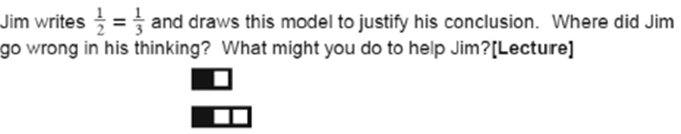
\includegraphics[width=0.6\textwidth]{kas_ne_taip2.png}
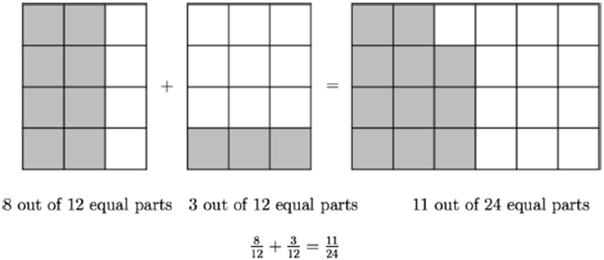
\includegraphics[width=0.4\textwidth]{kas_ne_taip1.png}

\subsection{Measurement (matavimas)} 
Šiame subkonstrukte trupmena yra glaustai susijusi su dviem sąvokomis: skaičius, atitinkantys tašką skaičių ašyje, ir skaičius, atitinkantis atkarpos ilgį.  Šis matavimo vaizdinys išvestas iš kiekinio trupmenos vaizdinio. Tai paaiškinama remiantis tokiu kategorizavimu: lyginimo atskiras tipas yra ilgių skaičių ašyje atidėjimas, o dalių atskiras tipas yra ilgiai. Žemiau pateikiamas vaizdinių palyginimas.\\ \\
\phantom{xxxxxxxxxx}\textbf{Kiekio trupmenos vaizdinys}\phantom{xxxxxxxxxxxxxxxxxxxxxxx}\textbf{Išvestas vaizdinys}\\ \\
\phantom{xxxxxxxxxxxxxxx}$\tikz[baseline]{\node(d30) {\boxed{\frac{\tikz[baseline]{\node(d28) {$a$}}}{\tikz[baseline]{\node(d29){$b$}}}}}}$
\begin{tikzpicture}[remember picture, overlay] %overlay parametras nurodo, kad paveikslėlis eis tiesiai iš lygties
%in yra įėjimo kampas, out yra išėjimo kampas (kur eis vektorius, priešingas įėjimo krypčiai; išėjimo krypties kampas)
%dėmenyje skliausteliuose: (pirmas narys= kampas, kuriuo slinksis tekstas; antras narys = jo nuotolis)
%atskaitos tašką nurodo north - t.y. kad rodyklė eis iš po teksto
%text width= paaiškinamo teksto plotis, align=center garantuoja, kad kėlimas į kitą eilutę leistinas
\draw[blue,thick,->] (d28) to [in=90,out=180] + (225:2.5cm) node[anchor=north,text = black, align=center] {kiek atskirtų dalių imame};
\draw[blue,thick,->] (d29) to [in=90,out=225] + (270:0.7cm) node[anchor=north,text = black, align=center] {į kiek dalių dalijame};
\draw[blue,thick,->] (d30) to [in=150,out=0] + (350:1.7cm) node[anchor=west,text = black, align=left] {atskirtą dalį atitinkančio\\ kiekio lyginimas su\\ visu suskaidytu kiekiu};
\end{tikzpicture}
\phantom{xxxxxxxxxxxxxxxxxxxxxxxxxxxxxxxxxxxxxxxxxxx}$\tikz[baseline]{\node(d28) {\boxed{\frac{\tikz[baseline]{\node(d26) {$a$}}}{\tikz[baseline]{\node(d27){$b$}}}}}}$
\begin{tikzpicture}[remember picture, overlay] %overlay parametras nurodo, kad paveikslėlis eis tiesiai iš lygties
%in yra įėjimo kampas, out yra išėjimo kampas (kur eis vektorius, priešingas įėjimo krypčiai; išėjimo krypties kampas)
%dėmenyje skliausteliuose: (pirmas narys= kampas, kuriuo slinksis tekstas; antras narys = jo nuotolis)
%atskaitos tašką nurodo north - t.y. kad rodyklė eis iš po teksto
%text width= paaiškinamo teksto plotis, align=center garantuoja, kad kėlimas į kitą eilutę leistinas
\draw[blue,thick,->] (d26) to [in=90,out=180] + (225:2.5cm) node[anchor=north,text = black, align=center] {kiek dalių imame};
\draw[blue,thick,->] (d27) to [in=90,out=225] + (320:0.8cm) node[anchor=north,text = black, align=center] {į kiek dalių dalijame sutartinį ilgį};
\draw[blue,thick,->] (d28) to [in=150,out=0] + (350:1.7cm) node[anchor=west,text = black, align=left] {gauto ilgio atidėjimas \\ (lyginamas su kitais\\ atidėtais ilgiais)};
\end{tikzpicture}\\ \\ \\ \\ \\ \\ \\ \\

\textbf{\textit{Mokiniams svarbu:}}
\begin{enumerate}
\item Atlikti šuolį nuo sveikų prie trupmeninių skaičių: iš pradžių jų vaizdinys konfliktiškas, nes trupmenomis nedalomų daiktų kiekiai neskaičiuojami. Šis konfliktas nuveda moksleivius į klaidingą trupmenų vaizdinį suvokiant jas kaip du skaičius ir lemia skaičiavimo klaidas, tokias kaip $\frac{1}{2}+\frac{1}{4}=\frac{2}{6}$. 
\item Gebėti panaudojant duotą intervalą rasti atstumą nuo pradžios taško. 
\item Įsitikinti, kad jų trupmenos vaizdinio suvokimas nėra klaidingas: skaičiuojant nepainioti brūkšniukų su intervalais.
\item APIBENDRINTAI –  būtina įsisąmoninti trupmenų išdėstymo eilės ir trupmenų ekvivalentumo aspektus.
\end{enumerate}

\subsection{Quotient (dalmuo)}
Šiame subkonstrukte trupmena interpretuojama kaip dalybos rezultatas. Taigi trupmenos vaizdinys yra išvestas dalijimo trupmenos vaizdinio. Verta paminėti, jog dalijimo trupmenos vaizdinys persidengia su dalybos vaizdiniu. Dažnai remiamasi konkrečiu vaizdiniu, kuomet dalmuo nurodo kiekvienam asmeniui tenkantį kiekį, o daliklis - asmenų, kuriems dalinama, kiekį, tačiau siekiama, kad trupmenos vaizdinio suvokimas turi tapti abstrakčiu. \textbf{\textit{Mokiniams svarbu:}}
\begin{enumerate}
\item Išmokti atsiriboti nuo vieno objekto dalijimo į lygias dalis ir pereiti prie keleto objektų dalijimo į keletą dalių.
\item Suprasti, kad skaitiklis gali būti mažesnis/lygus/didesnis nei vardiklis. Tuo pačiu dalmuo irgi gali būti mažesnis/lygus/didesnis už daliklį.
\item APIBENDRINTAI –  būtina suprasti dalybos proceso dvilypę struktūrą:  po kiek kokio dydžio dalių sudaro visumą, jei dalinama gali būti kokios tik nori struktūros į kiek tik nori dalių.
\end{enumerate}

\subsection{Operation (operacija)} Šiame vaizdinyje trupmena yra susijusi su procesu, vykstančiu keičiant skaičių, objektą ar aibę, o šio pokyčio rezultatas priklauso nuo trupmenos skaitiklio ir vardiklio. Taigi trupmena yra transformavimo priemonė (į tiesės/plokštumos kito dydžio segmentus ar didesnį/mažesnį aibės elementų kiekį). \textbf{\textit{Mokiniams svarbu:}}:
\begin{enumerate}
\item Trupmeninį daugiklį išmokti interpretuoti įvairiais būdais.
\item Įvardinti trupmeną, galinčią aprašyti sudėtinę operaciją .
\item Susieti operacijos duomenis su rezultatu.
\item APIBENDRINTAI –  įsivaizduoti ištempimą/suspaudimą išlaikant tą patį dalių kiekį arba išlaikant tą patį dalių dydį; taip pat pakeisti dalių kiekį.
\end{enumerate}

\subsection{Ratio (santykis)}
Šis subkonstruktas išreiškia dviejų dydžių palyginimą. Lyginimo rezultatas yra palyginimo rodiklis, simbolizuojantis proporciją. \textbf{\textit{Mokiniams svarbu:}}:
\begin{enumerate}
\item Sugebėti priskirti tinkamas prasme santykyje esantiems kiekiams.
\item Suvokti, kad du kiekiai santykyje galima keisti kartu taip, kad jų santykis išliktų nekintantis. 
\item Žinoti, kad santykyje esančius kiekius padauginus iš to paties skaičiaus, pats jų santykis išliks tas pats.
\item APIBENDRINTAI – išplėtoti trupmenų ekvivalentumo apibrėžimą.
\end{enumerate}

\subsection{Visų subkonstruktų apžvalga}

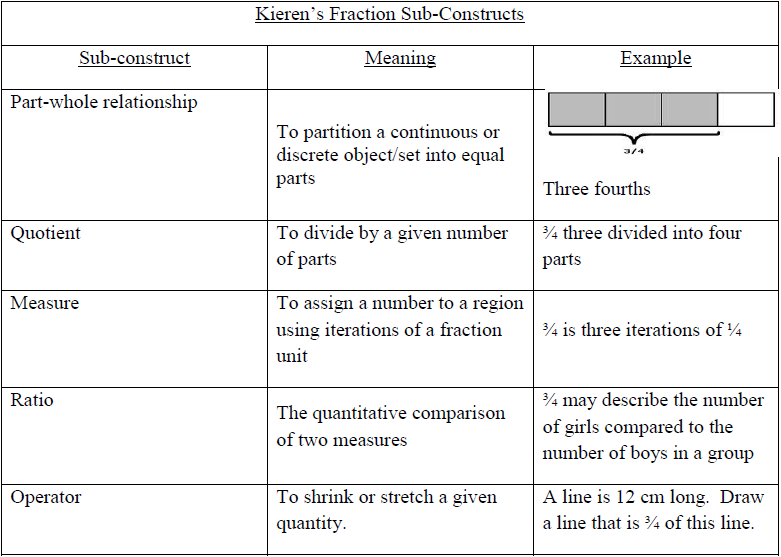
\includegraphics[width=0.8\textwidth]{kieglers_classify.png}
\begin{itemize}
\item Trupmenų mokymas naudojant tik vieną subkonstruktą, pavyzdžiui dalies/visumos, gali būti nepakankamas, kai susiduriama su kitais subkonstruktais. 
\item Moksleivių apypilimas keliais subkonstruktais vienu metu teigiant, kad jie visi tinkami apibūdinti tą patį skaičių $\frac{a}{b}$, gali būti per sudėtinga net ir gabiausiems moksleiviams.
\item Norint, kad bet kuris sėkmingui naujo subkonstrukto mokymas pavyktų, naujas požiūris į trupmeną turi būti pristatomas išryškinant, kaip jis dera su kitais subkonstruktais (kaip papildo, ar kaip yra išvestas iš kitų vaizdinių).
\item \textbf{\textit{Part-whole}} subkonstruktas persidengia su kitais subkonstruktais arba naudojamas išvesti kitiems subkonstruktams, todėl pažintį su trupmenomis patartina pradėti nuo jo.
\end{itemize}
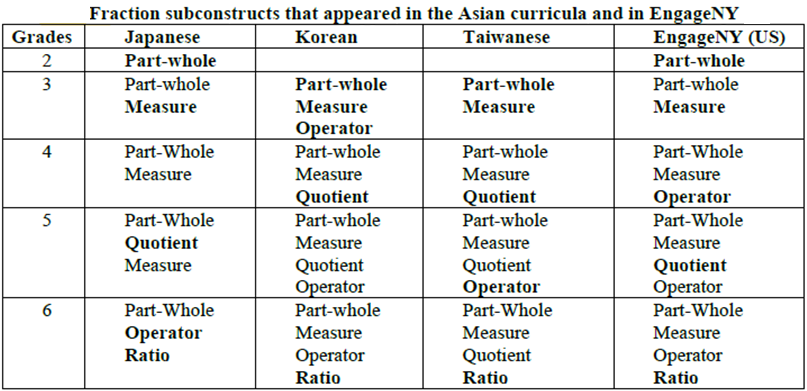
\includegraphics[width=0.8\textwidth]{sampratynas.png}

\subsection{Trupmenų vaizdinius iliustruojantys uždaviniai (16)}
\noindent\foreach \n in {2018/B2018/B2018_11.jpg, 2017/B2017/B2017_8.jpg, 2017/B2017/B2017_24.jpg, 2016/B2016/B2016_2.jpg, 2016/B2016/B2016_5.jpg, 2015/B2015/B2015_1.jpg, 2015/B2015/B2015_6.jpg, 2014/B2014/B2014_2.jpg, 2014/B2014/B2014_11.jpg, 2014/B2014/B2014_25.jpg, 2013/B2013/B2013_23.jpg, 2012/B2012/B2012_21.jpg, 2012/B2012/B2012_24.jpg, 2012/B2012/B2012_28.jpg, 2006/B2006/B2006_15.jpg, 2006/B2006/B2006_23.jpg}{\inc{\n}\\}
\subsection{Vaizdinius, persidengiančius su trupmenų vaizdiniais, iliustruojantys uždaviniai (23)}
\noindent\foreach \n in {2018/B2018/B2018_4.jpg, 2018/B2018/B2018_6.jpg, 2018/B2018/B2018_26.jpg, 2017/B2017/B2017_9.jpg, 2017/B2017/B2017_19.jpg, 2016/B2016/B2016_8.jpg, 2016/B2016/B2016_29.jpg, 2015/B2015/B2015_13.jpg, 2015/B2015/B2015_22.jpg, 2014/B2014/B2014_6.jpg, 2014/B2014/B2014_10.jpg, 2014/B2014/B2014_24.jpg, 2013/B2013/B2013_3.jpg, 2013/B2013/B2013_8.jpg, 2013/B2013/B2013_14.jpg, 2012/B2012/B2012_2.jpg, 2012/B2012/B2012_3.jpg, 2012/B2012/B2012_4.jpg, 2012/B2012/B2012_13.jpg, 2012/B2012/B2012_15.jpg, 2006/B2006/B2006_9.jpg, 2006/B2006/B2006_18.jpg, 2006/B2006/B2006_28.jpg}{\inc{\n}\\}
\newpage
\subsection{Uždaviniai Mantui iš įrašymų}
\noindent\foreach \n in {2018/B2018/B2018_29.jpg, 2018/B2018/B2018_27.jpg, 2018/B2018/B2018_13.jpg, 2018/B2018/B2018_16.jpg, 2018/B2018/B2018_21.jpg, 2018/B2018/B2018_25.jpg, 2017/B2017/B2017_28.jpg, 2017/B2017/B2017_22.jpg, 2017/B2017/B2017_15.jpg, 2017/B2017/B2017_11.jpg, 2017/B2017/B2017_7.jpg}{\inc{\n}\\}
\section{Aukštesnio lygio mąstymo uždaviniai ne iš Kengūros}
Kompetencijos, kurias reikia ugdyti 21 amžiuje:
\begin{itemize}
\item Kūrybiškumas
\item Gebėjimas tyrinėti ir atrasti naujus dalykus
\item Gebėjimas save nukreipti tinkama kryptimi, iniciatyvumas, atkaklumas
\item Gebėjimas naudotis informacija
\item Struktūruotas mąstymas
\item Gebėjimas komunikuoti
\item Samprotavimas
\end{itemize}
Analizuojant Matematika Tau 8 klasės vadovėlį pagal tai, kiek jo teorinėje medžiagoje, pateiktuose uždavinių sprendimo pavyzdžiuose ir uždavinių rinkiniuose reikalingas aukštesnio lygio mąstymas, paaiškėjo, kad tik 8 uždaviniuose iš 790 nagrinėtų tokių kompetencijų reikia.

Užduotėlių pavyzdžiai:
\begin{enumerate}
\item Virtuvė su trimis prietaisais ir trijomis rozetėmis. (Polya)
\item Duota $12^2+1^2+31^2$ ir $13^2+1^2+21^2=...$ Pratęskite lygybę. (Matematika Tau, 8kl.)
\item Paveikslėlyje pavaizduoti visi galimi erdviniai kūnai, kurių sienos yra taisyklingieji daugiakampiai:

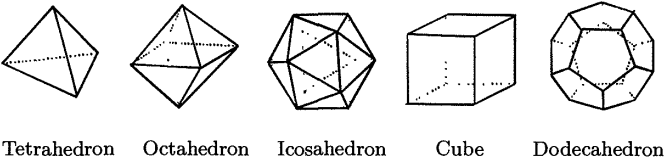
\includegraphics[width=0.6\textwidth]{edrai.png}

Samprotavimas susideda iš šių etapų:
\begin{itemize}
\item Duota piramidė, kurios visos sienos yra vienodi lygiašoniai trikampiai. Kaip keisis kampai jos sienose, jei piramidės viršūnę slinksime palei tiesę, kurioje yra šios piramidės aukštinė?
\item Tarkime, kad kažkuri viršūnė yra bendra su $n$ sienų. Kokias reikšmes gali įgyti sienų kampai, išeinantys iš tos viršūnės?
\item Kokiems taisyklingiesiems daugiakampiams tokie kampai galimi?
\end{itemize}
\item Duotas kvadratinis kiemas su apvaliais krūmais ir kvadratiniu baseinu. Kaip padidinti šio baseino plotą dvigubai, kad jis neitų per krūmus?
\item Trikampių lygumo požymiai. Nustatykime tris parametrus, kurie trikampyje yra nekintami. Ar aišku, kaip turint šiuos parametrus vienareikšmiškai gauti trikampį? Ar aišku, kaip trikampis gali būti slenkamas nekeičiant šių parametrų? Ar visada galima atlikti slinkimą, kad vienas trikampis sutaptų su kitu trikampiu, turinčiu tuos pačius parametrus?
\item Trikampių lygumo požymis pagal tris kraštines. Kaip turint tris duoto ilgio atkarpas iš jų sudaryti trikampį?
\item Funkcijų intelektinis poreikis. Kur pasitaiko mokyklinės funkcijos $3x+2$, $x^2$, $2^{-x}+2^x$, $\cos x$, $e^{-7x}$, $e^{-7x}\times \cos(x)$, $\frac{1}{x}$? Kur pasitaiko jų eskizai?
\item Masteliai. Išrikiuokime fizikinių objektų pavyzdžius didėjimo tvarka pradedant nuo mikropasaulio ir baigiant makropasauliu ir juos pavaizduokime sąsiuvinyje taip, kad būtų proporcingai išlaikomi stebimų objektų matmenys ir atstumai. Galima remtis atskirais faktais, kurie žinomi iš įvairios literatūros. 

Didelių išmatavimų pavyzdžiai.
\begin{itemize}
\item Atstumas nuo Žemės iki Mėnulio - kiek daugiau, nei šviessekundė. 
\item Žemės pusiaujas 40000 kilometrų. 
\item Jei į vieną eilę sudėtume 109 žemes, gautume Saulės skersmenį. 
\item Nuo Saulės iki Žemės šviesa sklinda 500 sekundžių ir nukeliauja 150mln. kilometrų
\end{itemize}
Mažų išmatavimų pavyzdžiai:
\begin{itemize}
\item Hadronų kolaideryje artišviesiniais greičiais priešpriešine kryptimi paleidžiamos atomus sudarančios dalelės ir joms susidūrus gaunamos kitos dalelės, iš kurių galima gauti informacijos apie pirmykštes daleles, sudariusias visatą.
\item Atomus sudaro branduolys su teigiamą krūvį turinčiomis dalelėmis (protonu ir neutronu), o aplink atomo branduolį įvairiomis orbitalėmis skrieja elektronai - neigiamą krūvį turinčios dalelės.
\item Elektronai skrieja taip greitai, kad galima būtų tik teoriškai nustatyti trajektorijas, kuriomis jie skries.  
\item Trajektorija yra tarsi šviesos pėdsakas, kurį mes galime pamatyti, kuomet mojuojame degančiu pagaliu tamsoje, tačiau nematome stabilios pagalio galo padėties. Žmogaus akis apdoroja informaciją ne daugiau, nei 24 kadrais per sekundę, todėl tankesni kadrai susilieja ir telieka (šviesos arba pravažiuojančio automobilio) pėdsakas.
\item Jei atomo branduolį įsivaizduotume kaip futbolo kamuolį, tai aplink jį skriejantis elektronas būtų už 50 kilometrų ir žirnio dydžio.
\item Medžiagą galima apibūdinti pagal tai, iš kokių atomų ji sudaryta. Pvz. vandens molekulė yra iš dviejų vandenilio ir vieno deguonies atomo.
\item Atomai turi pavadinimus. Pavyzdžiui azotas, deguonis, anglis, vandenilis. Jie skiriasi tik tuo, kad juos sudaro skirtingas atomų, neutronų ir elektronų kiekis.
\item Ore 78\% vietos užima azotas, 21\% deguonis ir apie 1\% - likusios medžiagos, tokios kaip argonas arba anglies dioksidas.
\item Molekulės - tai iš kelių atomų sudarytos dalelės. 
\item Sąlyginai nedidelis molekulių kiekis yra genuose. Genai sudaro ląstelės chromosomas, kurios yra ląstelės branduolyje, o branduolys yra vienas iš ląstelės organoidų.
\item Ląstelės sudaro skaidulas; skaidulos sudaro audinius, audiniai sudaro raumenis.
\end{itemize}
\item Perrinkite ir įvertinkite visus galimus variantus mano pateiktoje šaškių situacijoje
\item Duotas Paskalio trikampis. Ar galite pastebėti, kaip jis sudarytas ir ar mokate jį pratęsti? 
\item NIM žaidimas: raskite laiminčiuosius ir pralaiminčiuosius skaičius nuo 1 iki 30, kai duotajam skaičiui du žaidėjai gali iš šaškių krūvos imti tik pirminį skaičių šaškių.
\end{enumerate}
\newpage
\subsection{Kūrybiniai projektai}
Šiame straipsnyje išskirsime vietą ir keletui projektų, kurie turėtų atskleisti, kaip matematinės žinios gali būti taikomos sprendžiant realaus pasaulio problemas ir kaip šios žinios gali būti jungiamos su kitų dalykų žiniomis. Kiekvieno projekto tikslas - sužinoti kuo daugiau apie tai, kas vyksta erdvėje, kurios dar negalėjome pamatyti. Darant šį projektą matematinių gebėjimų nepakanka: jie neišvengiamai persipina su gebėjimais, kurių reikia mokantis kitus dalykus. Įgūdžiai, kuriuos įgysite atlikdami projekto užduotį, yra tokie:
\begin{itemize}
\item Taikyti matematines žinias įvertinant laiką, atstumą, greitį, temperatūrą ir daug kitų dydžių arba skaičių.
\item Mokytis kuo greičiau susirasti informaciją internete.
\item Plėsti kritinį mąstymą: nuolat kelti klausimus, vertinti, ar rasti atsakymai atitinka tikrovę.
\item Kompetencijos pojūtis: pasitikėjimas, įgytas radus atsakymus į klausimus, kylantis susidomėjimas, motyvacija, azartas ieškant atsakymų.
\end{itemize}
Verta paminėti, kad kiekvieno projekto tematika nenuspėjama, nes ji labiau priklauso ne nuo skaičiavimų, kuriuos norime išmokti atlikti, o nuo klausimų, kurie gali nuvesti tyrinėtoją netikėtomis kryptimis ir pareikalauti tokių žinių, kurios gali beveik nesisieti su užduoties pradžioje keltais klausimais.

Paryškintos nuorodos gerokai palengvins atsakymų į keliamus klausimus ieškojimą. Projektų autorius Simonas tikisi, jog po kurio laiko klausimų kėlimas ir žinojimas, kur ieškoti atsakymų į juos taps savaiminiu procesu. 
\subsection{Braškių laukai}
\subsection{Tarpgalaktinis skrydis}
\subsection{Plika akimis nematomi nuotoliai}
Tikslas. Kuo giliau pažinti procesus, kurie vyksta plika akimi nematomoje erdvėje ir atrasti objektų su nurodytais, bet plika akimi nematomais dydžiais, pavyzdžių.

Pradžia. \href{https://www.youtube.com/watch?v=7WhRJV\_bAiE}{\textcolor{blue}{Filmukas}} apie nematomą mažąjį pasaulį. Prieš leidžiantis į tyrinėjimus siūlome susipažinti su mikroskopinių ilgių \href{https://lt.wikipedia.org/wiki/Matavimo_vienetas#Ilgio_matavimo_vienetai}{\textcolor{blue}{matavimo vienetais}}. Daug išsamesnė informacija yra \href{https://en.wikipedia.org/wiki/Orders\_of\_magnitude\_(length)}{\textcolor{blue}{angliškoje Vikipedijoje}}.

Užduotys.
\begin{enumerate}
\item Sudarykite lentelę. Jos stulpeliuose turi būti užrašyti objektai ir jų dydžiai pradedant nuo didžiausio ir baigiant mažiausiu. Taip pat atskirame stulpelyje arba prie kiekvieno nurodyto objekto nurodykite, kiek jis kartų mažesnis už anksčiau paminėtą. Siūloma įtraukti šių objektų matmenis:\textit{galva, akis, plaukas, ląstelė, makroskaidula, mikroskaidula, protoskaidula, keratino molekulė, sieros, anglies, azoto ir deguonies atomai, elektrono orbitalės ilgis, orbitalės plotis, protonas, kvarkas}.
\item \href{\detokenize{https://lt.wikipedia.org/wiki/Ląstelė}}{\textcolor{blue}{Ląstelės}}. 
\begin{enumerate}
\item Išvardykite ląstelių \href{\detokenize{https://lt.wikipedia.org/wiki/Ląstelė#Prokariotų_ląstelių_struktūra}}{\textcolor{blue}{sudedamąsias dalis}}, kurios jums atrodo svarbiausios. Kaip jos vadinamos?
\item  Kaip ląstelės gauna medžiagų? 
\item Kas atitiktų ląstelės smegenis ir ką tos smegenys kontroliuoja? Kurioje ląstelės dalyje yra paveldima ląstelės informacija? 
\item \href{https://lt.wikipedia.org/wiki/Chromosoma}{\textcolor{blue}{Kas}} atitinka vieną žmogaus ląstelės atminties vienetą ir kiek žmogaus ląstelė jų turi? 
\item Koks yra šio atminties vieneto ilgis? 
\item \href{https://www.youtube.com/watch?v=V04jvRh5YFE}{\textcolor{blue}{Iš kokių dalelių}} ir \href{\detokenize{https://lt.wikipedia.org/wiki/Deoksiribonukleorūgštis}}{\textcolor{blue}{kokios medžiagos}} tas atminties vienetas sudarytas? 
\item \href{\detokenize{https://en.wikipedia.org/wiki/DNA}}{\textcolor{blue}{Kokia forma}} yra susivijusi šios medžiagos \href{\detokenize{https://lt.wikipedia.org/wiki/Molekulė}}{molekulė}? 
\item Kokio storio ji maždaug galėtų būti? 
\item Kas sudaro molekules ir kaip jos atrodo? Pavyzdžiui vandens molekulė? 
\item Kodėl tokios medžiagos, kaip baltymai yra vadinamos makromolekulėmis ir iš ko jos sudarytos? Ar $DNR$ yra taip pat makromolekulė? Ar nenusinuodytumėte paragavę kokių nors medžiagų makromolekulių?
\end{enumerate}
\item DNR ir paveldimumas. Akylas skaitytojas turėtų žvilgterti ir \href{https://lt.wikipedia.org/wiki/Deoksiribonukleorūgštis#Nuorodos}{\textcolor{blue}{šaltinius}}, kuriais remiasi dominantys Vikipedijos straipsniai. Šiuo atveju norodoje informacija labai \href{http://www.johnkyrk.com/chromosomestructure.lit.html}{\textcolor{blue}{išsami}} ir tinkama mūsų tyrimui. Taip pat pasidairius po angliškos Vikipedijos iliustracijas galima atrasti ir \href{https://en.wikipedia.org/wiki/DNA#Biological\_functions}{kitų išsamių iliustracijų}. Nauji klausimai, kuriuos galima išsikelti tiriant DNR:
\begin{enumerate}
\item Kokių matmenų yra \textit{ląstelė, jos branduolys, chromosoma, DNR}?
\item \href{https://lt.wikipedia.org/wiki/Genas}{\textcolor{blue}{Kas vaizduojama}} brūkšneliais, įeinančiais į DNR? 
\item Kiek genų būna žmogaus DNR? Kuri jų dalis atsakinga už paveldimumą? 
\item Naudojantis pateikta iliustracija galima gauti tokių duomenų: \textit{vienoje pilnoje spiralės apsukoje yra 10 bazių porų; apsukos ilgis siekia 34 atommetrus; apsukos plotis yra 20 atommetrų; tarp dviejų baltyminių sąrėd}
\end{enumerate}
\end{enumerate} 

\subsection{Aukštos įtampos laidai}
Tarp aukštosios elektros įtampos stulpų eina po tris laidininkus, tarp kurių teka srovė. Mechanikas Žilvinas po 6 val. skrydžio sraigtasparniu lazeriu nuskenavo 882 laidininkus, einančius tarp 295 stulpų. Tuo metu lauke buvo 20 laipsnių šilumos. Kiekvieno laidininko duomenys buvo įrašyti į duomenų failą. Laidininko duomenis sudaro 20, 30 arba 40 vienodais tarpais išdėstytų taškų ir kiekvienam taškui užrašyta jo koordinatės žemės atžvilgiu bei aukštis:

\begin{minted}{text}
Vertices=40 Hole=0 Level=17 Color=-1 Weight=-1 Style=2147483647 Reference=0
566014.7604 6575670.0925 52.5728
566016.8032 6575663.6837 51.9256
566018.8461 6575657.2748 51.3135
566020.8889 6575650.8659 50.7367
566022.9318 6575644.4571 50.1951
...
\end{minted}

Darbdavys matematiko Simono paklausė, ar jis sugebėtų pagal aukščiau pateiktus 40 taškų, per kuriuos eina laidininkas, apskaičiuoti funkciją, skirtą nustatyti laidininko aukštį bet kuriame (nebūtinai duotame) jo taške. Į tai Simonas atsakė: \textit{man užtektų ir trijų taškų. Spėju, jog mano teoriškai gauta funkcija būtų pakankamai tiksli, o pagal likusių 37 taškų koordinates būtų galima įvertinti, kiek mano skaičiavimai apsirinka.}

Po savaitės darbo Simono spėjimai pasitvirtino. Jis parašė programą, kuri per dvi minutes kiekvienam iš 882 laidininkų ne tik suranda funkciją, bet ir nustato, kaip pasikeistų duotų 40 taškų koordinatės, kai laidininkas įšiltų ligi 35 arba 70 laipsnių. Paleidus programą apskaičiuotos kiekvieno taško trimatės koordinatės yra įrašomos į naujai sukurtą .txt failą. Ši programa vėliau bus naudojama aplikacijoje, kuri kreipiasi Komandinę eilutę (Command Prompt) ir leidžia pamatyti apskaičiuotas laidų padėtis erdvėje (panašiai kaip žaidžiant kompiuterinį žaidimą).

\subsection{Garso bangos}
\newpage
\section{grafai, medžiai ir variantai}
\noindent\foreach \n in {2018/B2018/B2018_15.jpg, 2018/B2018/B2018_17.jpg, 2018/B2018/B2018_21.jpg, 2018/B2018/B2018_23.jpg, 2017/B2017/B2017_5.jpg, 2017/B2017/B2017_7.jpg, 2017/B2017/B2017_12.jpg, 2017/B2017/B2017_20.jpg, 2017/B2017/B2017_26.jpg, 2017/B2017/B2017_29.jpg, 2017/B2017/B2017_30.jpg}{\inc{\n}\\}

\end{document}